\section{Arquitecturas ILP}

\begin{ejercicio} \label{ej:1_R4}
    Considere el fragmento de Código~\ref{cod:ej1_R4}.
    \begin{listing}[H]
    \begin{minted}[xleftmargin=4cm, linenos]{asm}
lw  r1,0x1ac    ; r1 <-- M(0x1ac)
lw  r2,0xc1f    ; r2 <-- M(0xc1f)
add r3,r0,r0    ; r3 <-- r0+r0
mul r4,r2,r1    ; r4 <-- r2*r1
add r3,r3,r4    ; r3 <-- r3+r4
add r5,r0,0x1ac ; r5 <-- r0+0x1ac
add r6,r0,0xc1f ; r6 <-- r0+0xc1f
sub r5,r5,#4    ; r5 <-- r5 - 4
sub r6,r6,#4    ; r6 <-- r6 - 4
sw  (r5),r3     ; M(r5) <-- r3
sw  (r6),r4     ; M(r6) <-- r4
    \end{minted}
    \caption{Código para trabajar.}
    \label{cod:ej1_R4}
\end{listing}
Suponiendo que se pueden captar, decodificar, y emitir cuatro instrucciones por ciclo, indique el orden en que se emitirán las instrucciones para cada uno de los siguientes casos:
\begin{enumerate}
    \item Una ventana de instrucciones centralizada con emisión ordenada.
    
    Se encuentra resuelto en la Tabla~\ref{tab:ej1_R4_1}.
    \item Una ventana de instrucciones centralizada con emisión desordenada.
    
    Se encuentra resuelto en la Tabla~\ref{tab:ej1_R4_2}.
    \item Una estación de reserva de tres líneas para cada unidad funcional, con envío ordenado.

    Se encuentra resuelto en la Tabla~\ref{tab:ej1_R4_3}.
\end{enumerate}

Nota: considere que hay una unidad funcional para la carga (2 ciclos), otra para el almacenamiento (1 ciclo), tres para la suma/resta (1 ciclo), y una para la multiplicación (4 ciclos). También puede considerar que, en la práctica, no hay límite para el número de instrucciones que pueden almacenarse en la ventana de instrucciones o en el buffer de instrucciones.\\

Según el enunciado del ejercicio, el cauce de instrucciones tiene la siguiente forma:
\begin{figure}[H]
\centering
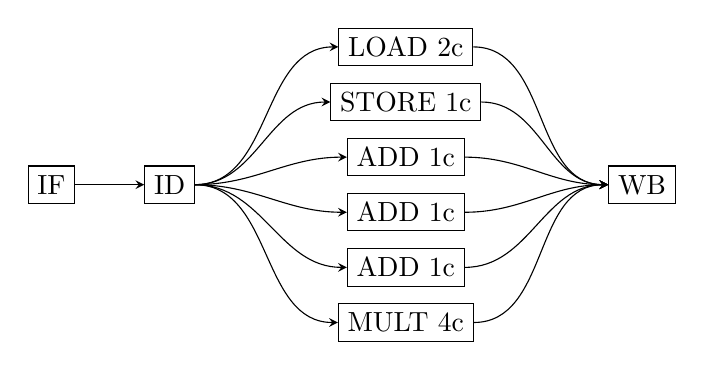
\begin{tikzpicture}
    \node[draw, rectangle] (A) at (-0.5,1.75) {IF};
    \node[draw, rectangle] (B) at (1,1.75) {ID};

    \node[draw, rectangle] (C) at (4,3.5) {LOAD 2c};
    \node[draw, rectangle] (D) at (4,2.8) {STORE 1c};
    \node[draw, rectangle] (E) at (4,2.1) {ADD 1c};
    \node[draw, rectangle] (F) at (4,1.4) {ADD 1c};
    \node[draw, rectangle] (G) at (4,0.7) {ADD 1c};
    \node[draw, rectangle] (H) at (4,0) {MULT 4c};

    \node[draw, rectangle] (I) at (7,1.75) {WB};

    \draw[-stealth] (A) -- (B);
    \draw[-stealth] (B) to[out=0,in=180] (C);
    \draw[-stealth] (B) to[out=0,in=180] (D);
    \draw[-stealth] (B) to[out=0,in=180] (E);
    \draw[-stealth] (B) to[out=0,in=180] (F);
    \draw[-stealth] (B) to[out=0,in=180] (G);
    \draw[-stealth] (B) to[out=0,in=180] (H);
    \draw[-stealth] (C) to[out=0,in=180] (I);
    \draw[-stealth] (D) to[out=0,in=180] (I);
    \draw[-stealth] (E) to[out=0,in=180] (I);
    \draw[-stealth] (F) to[out=0,in=180] (I);
    \draw[-stealth] (G) to[out=0,in=180] (I);
    \draw[-stealth] (H) to[out=0,in=180] (I);
\end{tikzpicture}
\end{figure}

Además, para cada caso, se ha desarrollado una tabla que muestra la evolución de la ejecución del código según el número de ciclos.

\begin{table}
\centering
\scriptsize
\begin{tabular}{|l|c|c|c|c|c|c|c|c|c|c|c|c|c|c|}
    \hline
    Instrucción / Ciclos & 1 & 2 & 3 & 4 & 5 & 6 & 7 & 8 & 9 & 10 & 11 & 12  & 13 & 14 \\
    \hline
    \verb|lw  r1, 0x1ac|     & IF & ID & EX & EX & & & & & & & & & & \\
    \hline        
    \verb|lw  r2, 0xc1f|     & IF & ID & & & EX & EX & & & & & & & & \\
    \hline           
    \verb|add r3, r0, r0|    & IF & ID & & & EX & & & & & & & & & \\
    \hline                        
    \verb|mul r4, r2, r1|    & IF & ID & & & & & EX & EX & EX & EX & & & & \\
    \hline            
    \verb|add r3, r3, r4|    & & IF & ID & & & & & & & & EX & & & \\
    \hline            
    \verb|add r5, r0, 0x1ac| & & IF & ID & & & & & & & & EX & & & \\
    \hline            
    \verb|add r6, r0, 0xc1f| & & IF & ID & & & & & & & & EX & & & \\
    \hline        
    \verb|sub r5, r5, #4|    & & IF & ID & & & & & & & & & EX & & \\
    \hline
    \verb|sub r6, r6, #4|    & & & IF & ID & & & & & & & & EX & & \\
    \hline
    \verb|sw  (r5), r3|      & & & IF & ID & & & & & & & & & EX & \\
    \hline          
    \verb|sw  (r6), r4|      & & & IF & ID & & & & & & & & & & EX \\
    \hline
\end{tabular}
\caption{Ejecución con ventana centralizada y emisión ordenada del Ejercicio~\ref{ej:1_R4}.}
\label{tab:ej1_R4_1}
\end{table}

\begin{table}
\centering
\scriptsize
\begin{tabular}{|l|c|c|c|c|c|c|c|c|c|c|c|c|}
    \hline
    Instrucción / Ciclos & 1 & 2 & 3 & 4 & 5 & 6 & 7 & 8 & 9 & 10 & 11 & 12  \\
    \hline
    \verb|lw  r1, 0x1ac|     & IF & ID & EX & EX & & & & & & & & \\
    \hline        
    \verb|lw  r2, 0xc1f|     & IF & ID & & & EX & EX & & & & & & \\
    \hline           
    \verb|add r3, r0, r0|    & IF & ID & EX & & & & & & & & & \\
    \hline                        
    \verb|mul r4, r2, r1|    & IF & ID & & & & & EX & EX & EX & EX & & \\
    \hline            
    \verb|add r3, r3, r4|    & & IF & ID & & & & & & & & EX & \\
    \hline
    \verb|add r5, r0, 0x1ac| & & IF & ID & EX & & & & & & & & \\
    \hline
    \verb|add r6, r0, 0xc1f| & & IF & ID & EX & & & & & & & & \\
    \hline
    \verb|sub r5, r5, #4|    & & IF & ID & & EX & & & & & & & \\
    \hline            
    \verb|sub r6, r6, #4|    & & & IF & ID & EX & & & & & & & \\
    \hline
    \verb|sw  (r5), r3|      & & & IF & ID & & & & & & &  & EX \\
    \hline
    \verb|sw  (r6), r4|      & & & IF & ID & & & & & & & EX &  \\
    \hline
\end{tabular}
\caption{Ventana centralizada y emisión desordenada del Ejercicio~\ref{ej:1_R4}.}
\label{tab:ej1_R4_2}
\end{table}

\begin{table}
\centering
\scriptsize
\begin{tabular}{|l|c|c|c|c|c|c|c|c|c|c|c|c|c|}
    \hline
    Instrucción / Ciclos & 1 & 2 & 3 & 4 & 5 & 6 & 7 & 8 & 9 & 10 & 11 & 12 & 13 \\
    \hline
    \verb|lw  r1, 0x1ac|     & IF & ID & EX & EX & & & & & & & & & \\
    \hline        
    \verb|lw  r2, 0xc1f|     & IF & ID & & & EX & EX & & & & & & & \\
    \hline           
    \verb|add r3, r0, r0| ~~(1)    & IF & ID & EX & & & & & & & & & & \\
    \hline                        
    \verb|mul r4, r2, r1|    & IF & ID & & & & & EX & EX & EX & EX & & & \\
    \hline            
    \verb|add r3, r3, r4| ~~(2)    & & IF & ID & & & & & & & & EX & & \\
    \hline
    \verb|add r5, r0, 0x1ac| ~~(3) & & IF & ID & EX & & & & & & & & & \\
    \hline
    \verb|add r6, r0, 0xc1f| ~~(1) & & IF & ID & EX & & & & & & & & & \\
    \hline
    \verb|sub r5, r5, #4| ~~(3)    & & IF & ID & & EX & & & & & & & & \\
    \hline            
    \verb|sub r6, r6, #4| ~~(1)    & & & IF & ID & EX & & & & & & & & \\
    \hline
    \verb|sw  (r5), r3|      & & & IF & ID & & & & & & & & EX & \\
    \hline
    \verb|sw  (r6), r4|      & & & IF & ID & & & & & & & & & EX \\
    \hline
\end{tabular}
\caption{Ejecución con ventanas repartidas y emisión ordenada del Ejercicio~\ref{ej:1_R4}.}
\label{tab:ej1_R4_3}
\end{table}

\end{ejercicio}

\begin{ejercicio}  \label{ej:2_R4}
    Cosidere el fragmento de Código~\ref{cod:ej2_R4}.
    \begin{listing}[H]
    \begin{minted}[xleftmargin=4cm, linenos]{asm}
lw   r3,0x10a   ; r3 <-- M(0x10a)
addi r2,r0,#128 ; r2 <-- r0+128
add  r1,r0,0x0a ; r1 <-- r0+0x0a
lw   r4,0(r1)   ; r4 <-- M(r1)
lw   r5,-8(r1)  ; r5 <-- M(r1-8)
mult r6,r5,r3   ; r6 <-- r5*r3
add  r5,r6,r3   ; r5 <-- r6+r3
add  r6,r4,r3   ; r6 <-- r4+r3
sw   0(r1),r6   ; M(r1) <-- r5
sw   -8(r1),r5  ; M(r1-8) <-- r5
sub  r2,r2,#16  ; r2 <-- r2-16
    \end{minted}
    \caption{Código para trabajar.}
    \label{cod:ej2_R4}
    \end{listing}
Suponga que se ejecuta en un procesador superescalar que es capaz de captar 4 instrucciones/ciclo, de decodificar 2 instrucciones/ciclo; de emitir utilizando una ventana de instrucciones centralizada 2 instrucciones/ciclo; de escribir hasta 2 resultados/ciclo en los registros correspondientes (registros de reorden, o registros de la arquitectura según el caso), y completar (o retirar) hasta 3 instrucciones/ciclo.

Indique el número de ciclos que tardaría en ejecutarse el programa suponiendo finalización ordenada y:
\begin{enumerate}
    \item Emisión ordenada.
    
    Se encuentra resuelto en la Tabla~\ref{tab:ej2_R4_1}.
    \item Emisión desordenada.
    
    Se encuentra resuelto en la Tabla~\ref{tab:ej2_R4_2}. Notemos que, como
    no pueden escribir en el ROB más de una instrucción por ciclo,
    la instrucción \verb|sub r2,r2,#16| ha de esperar un ciclo más.
\end{enumerate}
Nota: Considere que tiene una unidad funcional de carga (2 ciclos), una de almacenamiento (1 ciclo), tres unidades de suma/resta (1 ciclo), y una de multiplicación (6 ciclos), y que no hay limitaciones para el número de líneas de la cola de instrucciones, ventana de instrucciones, buffer de reorden, puertos de lectura/escritura etc.


Según el enunciado del ejercicio, el cauce de instrucciones tiene la siguiente forma:
\begin{figure}[H]
\centering
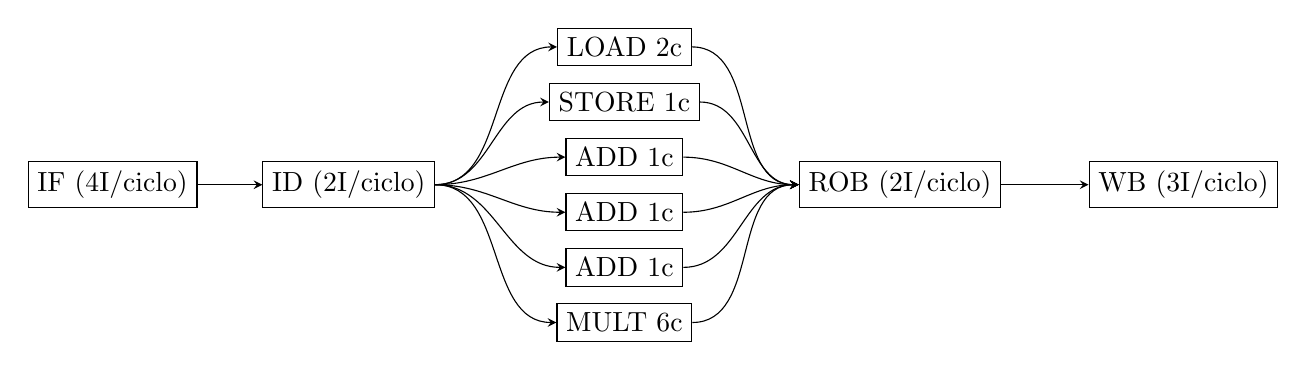
\begin{tikzpicture}
    \node[draw, rectangle] (A) at (-2.5,1.75) {IF (4I/ciclo)};
    \node[draw, rectangle] (B) at (00.5,1.75) {ID (2I/ciclo)};

    \node[draw, rectangle] (C) at (4,3.5) {LOAD 2c};
    \node[draw, rectangle] (D) at (4,2.8) {STORE 1c};
    \node[draw, rectangle] (E) at (4,2.1) {ADD 1c};
    \node[draw, rectangle] (F) at (4,1.4) {ADD 1c};
    \node[draw, rectangle] (G) at (4,0.7) {ADD 1c};
    \node[draw, rectangle] (H) at (4,0) {MULT 6c};

    \node[draw, rectangle] (I) at (7.5,1.75) {ROB (2I/ciclo)};
    \node[draw, rectangle] (J) at (11.1,1.75) {WB (3I/ciclo)};

    \draw[-stealth] (A) -- (B);
    \draw[-stealth] (B) to[out=0,in=180] (C);
    \draw[-stealth] (B) to[out=0,in=180] (D);
    \draw[-stealth] (B) to[out=0,in=180] (E);
    \draw[-stealth] (B) to[out=0,in=180] (F);
    \draw[-stealth] (B) to[out=0,in=180] (G);
    \draw[-stealth] (B) to[out=0,in=180] (H);
    \draw[-stealth] (C) to[out=0,in=180] (I);
    \draw[-stealth] (D) to[out=0,in=180] (I);
    \draw[-stealth] (E) to[out=0,in=180] (I);
    \draw[-stealth] (F) to[out=0,in=180] (I);
    \draw[-stealth] (G) to[out=0,in=180] (I);
    \draw[-stealth] (H) to[out=0,in=180] (I);
    \draw[-stealth] (I) to[out=0,in=180] (J);
\end{tikzpicture}
\end{figure}


\begin{table}
    \centering
    \scriptsize
    \begin{tabular}{|l|c|c|c|c|c|c|c|c|c|c|c|c|}
        \hline
        Instrucción / Ciclos & 1 & 2 & 3 & 4 & 5 & 6 & 7 & 8 & 9 & 10 & 11 & 12 \\
        \hline
        \verb|lw   r3,0x10a|        & IF & ID & EX & EX & ROB & WB & & & & & &\\
        \hline        
        \verb|addi r2,r0,#128|      & IF & ID & EX & ROB & & WB & & & & & &\\
        \hline           
        \verb|add  r1,r0,0x0a|      & IF & & ID & EX & ROB & WB & & & & & &\\
        \hline                        
        \verb|lw   r4,0(r1)|        & IF & & ID & & EX & EX & ROB & WB & & & &\\
        \hline            
        \verb|lw   r5,-8(r1)|       & & IF & & ID & & & EX & EX & ROB & WB & &\\
        \hline
        \verb|mult r6,r5,r3|        & & IF & & ID & & & & & EX & EX & EX & EX \\
        \hline
        \verb|add  r5,r6,r3|        & & IF & & & ID & & & & & & &\\
        \hline
        \verb|add  r6,r4,r3|        & & IF & & & ID & & & & & & &\\
        \hline            
        \verb|sw   0(r1),r6|        & & & IF & & & ID & & & & & &\\
        \hline
        \verb|sw  -8(r1),r5|        & & & IF & & & ID & & & & & &\\
        \hline
        \verb|sub  r2,r2,#16|       & & & IF & & & & ID & & & & &\\
        \hline \\ \hline \\ \hline
        \hline
        Instrucción / Ciclos & 13 & 14 & 15 & 16 & 17 & 18 & 19 \\
        \hline
        \verb|lw   r3,0x10a|        & & & & & & &\\
        \hline        
        \verb|addi r2,r0,#128|      & & & & & & &\\
        \hline           
        \verb|add  r1,r0,0x0a|      & & & & & & &\\
        \hline                        
        \verb|lw   r4,0(r1)|        & & & & & & &\\
        \hline            
        \verb|lw   r5,-8(r1)|       & & & & & & &\\
        \hline
        \verb|mult r6,r5,r3|        & EX & EX & ROB & WB & & & \\
        \hline
        \verb|add  r5,r6,r3|        & & & EX & ROB & WB & & \\
        \hline
        \verb|add  r6,r4,r3|        & & & EX & ROB & WB & & \\
        \hline            
        \verb|sw   0(r1),r6|        & & & & EX & ROB & WB & \\
        \hline
        \verb|sw  -8(r1),r5|        & & & & & EX & ROB & WB \\
        \hline
        \verb|sub  r2,r2,#16|       & & & & & EX & ROB & WB\\
        \hline
    \end{tabular}
    \caption{Emisión ordenada del código del Ejercicio~\ref{ej:2_R4}.}
    \label{tab:ej2_R4_1}
\end{table}

\begin{table}
    \centering
    \scriptsize
    \begin{tabular}{|l|c|c|c|c|c|c|c|c|c|c|c|c|}
        \hline
        Instrucción / Ciclos & 1 & 2 & 3 & 4 & 5 & 6 & 7 & 8 & 9 & 10 & 11 & 12 \\
        \hline
        \verb|lw   r3,0x10a|        & IF & ID & EX & EX & ROB & WB & & & & & &\\
        \hline        
        \verb|addi r2,r0,#128|      & IF & ID & EX & ROB & & WB & & & & & &\\
        \hline           
        \verb|add  r1,r0,0x0a|      & IF & & ID & EX & ROB & WB & & & & & &\\
        \hline                        
        \verb|lw   r4,0(r1)|        & IF & & ID & & EX & EX & ROB & WB & & & &\\
        \hline            
        \verb|lw   r5,-8(r1)|       & & IF & & ID & & & EX & EX & ROB & WB & &\\
        \hline
        \verb|mult r6,r5,r3|        & & IF & & ID & & & & & EX & EX & EX & EX \\
        \hline
        \verb|add  r5,r6,r3|        & & IF & & & ID & & & & & & &\\
        \hline
        \verb|add  r6,r4,r3|        & & IF & & & ID & & EX & ROB & & & &\\
        \hline            
        \verb|sw   0(r1),r6|        & & & IF & & & ID & & EX & ROB & & &\\
        \hline
        \verb|sw  -8(r1),r5|        & & & IF & & & ID & & & & & &\\
        \hline
        \verb|sub  r2,r2,#16|       & & & IF & & & & ID & EX & & \red{ROB} & &\\
        \hline \\ \hline \\ \hline
        \hline
        Instrucción / Ciclos & 13 & 14 & 15 & 16 & 17 & 18 & 19 \\
        \hline
        \verb|lw   r3,0x10a|        & & & & & & &\\
        \hline        
        \verb|addi r2,r0,#128|      & & & & & & &\\
        \hline           
        \verb|add  r1,r0,0x0a|      & & & & & & &\\
        \hline                        
        \verb|lw   r4,0(r1)|        & & & & & & &\\
        \hline            
        \verb|lw   r5,-8(r1)|       & & & & & & &\\
        \hline
        \verb|mult r6,r5,r3|        & EX & EX & ROB & WB & & & \\
        \hline
        \verb|add  r5,r6,r3|        & & & EX & ROB & WB & & \\
        \hline
        \verb|add  r6,r4,r3|        & & & & & \red{WB} & & \\
        \hline            
        \verb|sw   0(r1),r6|        & & & & & WB & & \\
        \hline
        \verb|sw  -8(r1),r5|        & & & & EX & ROB & WB & \\
        \hline
        \verb|sub  r2,r2,#16|       & & & & & & WB & \\
        \hline
    \end{tabular}
    \caption{Emisión desordenada del código del Ejercicio~\ref{ej:2_R4}.}
    \label{tab:ej2_R4_2}
\end{table}

\end{ejercicio}

\begin{ejercicio}\label{ej:3_R4}
   En el problema anterior: 
   \begin{enumerate}
       \item Indique qué mejoras realizaría en el procesador para reducir el tiempo de ejecución en la mejor de las opciones sin cambiar el diseño de las unidades funcionales (multiplicador, sumador, etc.) y sin cambiar el tipo de memorias ni la interfaz entre procesador y memoria (no varía el número de instrucciones captadas por ciclo).
       
       En primer lugar, consideramos que se decodifican el mismo número de instrucciones que se captan,
       eliminante el cuello de botella en la decodificación que teníamos en el problema anterior.
       Además, consideramos que no hay límite en el número de instrucciones por ciclo que se emiten, escriben en el ROB o completan.
       Por último, consideramos que disponemos de tantas unidades funcionales como se necesiten, para evitar así riesgos estructurales.
       Con estas mejoras, hemos llegado a la tabla~\ref{tab:ej3_R4_1}.
       
       \item ¿Qué pasaría si además se reduce el tiempo de multiplicación a la mitad?
       
       Resuelto en la tabla~\ref{tab:ej3_R4_2}. En este caso, tenemos una latencia inicial de $6$
       ciclos de reloj. Sabiendo que se ejecutan $11$ instrucciones en $12$ ciclos de reloj,
       tenemos que:
       \begin{equation*}
        T(n) = 12 = TLI + (n-1)CPI = 6 + (11-1)CPI \Rightarrow CPI = \frac{12-6}{11-1} = \frac{6}{10} = 0.6
       \end{equation*}

       Como $CPI=0.6<1$, podemos decir que el procesador es superescalar, pero no se trata de su
       mejor versión, ya que podemos llegar incluso a $3$ instrucciones por ciclo.
   \end{enumerate}
   
    \begin{table}
        \centering
        \scriptsize
        \begin{tabular}{|l|c|c|c|c|c|c|c|c|c|c|c|c|}
            \hline
            Instrucción / Ciclos & 1 & 2 & 3 & 4 & 5 & 6 & 7 & 8 & 9 & 10 & 11 & 12 \\
            \hline
            \verb|lw   r3,0x10a|        & IF & ID & EX & EX & ROB & WB & & & & & &\\
            \hline        
            \verb|addi r2,r0,#128|      & IF & ID & EX & ROB & & WB & & & & & &\\
            \hline           
            \verb|add  r1,r0,0x0a|      & IF & ID & EX & ROB & &  WB & & & & & & \\
            \hline                        
            \verb|lw   r4,0(r1)|        & IF & ID & & EX & EX & ROB & WB & & & & & \\
            \hline            
            \verb|lw   r5,-8(r1)|       & & IF & ID & EX & EX & ROB & WB & & & && \\
            \hline
            \verb|mult r6,r5,r3|        & & IF & ID & & & EX & EX & EX & EX & EX & EX & ROB\\
            \hline
            \verb|add  r5,r6,r3|        & & IF & ID & & & & & & & & & EX\\
            \hline
            \verb|add  r6,r4,r3|        & & IF & ID & & & EX & ROB & & & & &\\
            \hline            
            \verb|sw   0(r1),r6|        & & & IF & ID & & & EX & ROB & & & & \\
            \hline
            \verb|sw  -8(r1),r5|        & & & IF & ID & & & & & & & &\\
            \hline
            \verb|sub  r2,r2,#16|       & & & IF & ID & EX & & & & & & & \\
            \hline \\ \hline \\ \hline
            \hline
            Instrucción / Ciclos & 13 & 14 & 15 & 16 & 17 & 18 & 19 \\
            \hline
            \verb|lw   r3,0x10a|        & & & & & & &\\
            \hline        
            \verb|addi r2,r0,#128|      & & & & & & &\\
            \hline           
            \verb|add  r1,r0,0x0a|      & & & & & & &\\
            \hline                        
            \verb|lw   r4,0(r1)|        & & & & & & &\\
            \hline            
            \verb|lw   r5,-8(r1)|       & & & & & & &\\
            \hline
            \verb|mult r6,r5,r3|        & WR & & & & & & \\
            \hline
            \verb|add  r5,r6,r3|        & ROB & WB & & & & &\\
            \hline
            \verb|add  r6,r4,r3|        & & WB & & & & & \\
            \hline            
            \verb|sw   0(r1),r6|        & & WB & & & & & \\
            \hline
            \verb|sw  -8(r1),r5|        & EX & ROB & WB & & & & \\
            \hline
            \verb|sub  r2,r2,#16|       & & & WB & & & & \\
            \hline
        \end{tabular}
        \caption{Emisión desordenada del código de las mejoras Ejercicio~\ref{ej:2_R4}.}
        \label{tab:ej3_R4_1}
    \end{table}

    \begin{table}
        \centering
        \scriptsize
        \begin{tabular}{|l|c|c|c|c|c|c|c|c|c|c|c|c|}
            \hline
            Instrucción / Ciclos & 1 & 2 & 3 & 4 & 5 & 6 & 7 & 8 & 9 & 10 & 11 & 12 \\
            \hline
            \verb|lw   r3,0x10a|        & IF & ID & EX & EX & ROB & WB & & & & & &\\
            \hline        
            \verb|addi r2,r0,#128|      & IF & ID & EX & ROB & & WB & & & & & &\\
            \hline           
            \verb|add  r1,r0,0x0a|      & IF & ID & EX & ROB & &  WB & & & & & & \\
            \hline                        
            \verb|lw   r4,0(r1)|        & IF & ID & & EX & EX & ROB & WB & & & & & \\
            \hline            
            \verb|lw   r5,-8(r1)|       & & IF & ID & EX & EX & ROB & WB & & & && \\
            \hline
            \verb|mult r6,r5,r3|        & & IF & ID & & & EX & EX & EX & ROB & WR & & \\
            \hline
            \verb|add  r5,r6,r3|        & & IF & ID & & & & & & EX & ROB & WR & \\
            \hline
            \verb|add  r6,r4,r3|        & & IF & ID & & & EX & ROB & & & & WR &\\
            \hline            
            \verb|sw   0(r1),r6|        & & & IF & ID & & & EX & ROB & & & WR & \\
            \hline
            \verb|sw  -8(r1),r5|        & & & IF & ID & & & & & & EX & ROB & WB\\
            \hline
            \verb|sub  r2,r2,#16|       & & & IF & ID & EX & & & & & & & WB \\
            \hline
        \end{tabular}
        \caption{Emisión desordenada reduciendo la multiplicación del Ejercicio~\ref{ej:2_R4}.}
        \label{tab:ej3_R4_2}
    \end{table}
\end{ejercicio}

\begin{ejercicio}
    En el caso descrito en el problema~\ref{ej:3_R4}, indique cómo evolucionaría el buffer de reorden utilizado para implementar finalización ordenada, en la mejor de las opciones. 
\end{ejercicio}

\begin{ejercicio}
    En un procesador superescalar con renombramiento de registros se utiliza un buffer de renombramiento para implementar el mismo. Indique como evolucionarían los registros de renombramiento al realizar el renombramiento para las instrucciones del Código~\ref{cod:e5_R4}.
   \begin{listing}[H]
   \begin{minted}[xleftmargin=4cm, linenos]{asm}
mul r2, r0, r1  ; r2 <-- r0*r1
add r3,r1,r2    ; r3 <-- r1+r2
sub r2,r0,r1    ; r2 <-- r0-r1
add r3,r3,r2    ; r3 <-- r3+r2
   \end{minted}
   \caption{Instrucciones para renombrar}
   \label{cod:e5_R4}
   \end{listing}
\end{ejercicio}

\begin{ejercicio}\label{ej:6_R4}
    Considere el bucle del Código~\ref{cod:ej6_R4}.
    \begin{listing}[H]
    \begin{minted}[xleftmargin=4cm, linenos]{c}
i=1;
do
{
    b[i]=a[i]*c;
    c=c+1;
    if (c>10) then goto etiqueta; // 1
    i=i+1;
} while (i<=10); // 2
etiqueta: //..
    \end{minted}
    \caption{Bucle a considerar.}
    \label{cod:ej6_R4}
    \end{listing}

Indique cuál es la penalización efectiva debida a los saltos, en función del valor inicial de \verb|c| (número entero), considerando que el procesador utiliza:
\begin{enumerate}
    \item Predicción fija (siempre se considera que se va a producir el salto).
    \item Predicción estática (si el desplazamiento es negativo se toma y si es positivo no).
    \item Predicción dinámica con un bit (\verb|1=Saltar|; \verb|0=No Saltar|; Inicialmente está a 1).
\end{enumerate}
Nota: La penalización por saltos incorrectamente predichos es de 4 ciclos y para los saltos correctamente predichos es 0 ciclos.
\end{ejercicio}

\begin{ejercicio}
    En la situación descrita en el problema~\ref{ej:6_R4}. ¿Cuál de los tres esquemas es más eficaz por término medio si hay un 25\% de probabilidades de que c sea menor o igual a 0, un 30\% de que sea mayor o igual a 10; y un 45\% de que sea cualquier número entre 1 y 9, siendo todos equiprobables? 
\end{ejercicio}

\begin{ejercicio}
En un programa, una instrucción de salto condicional (a una dirección de salto anterior) dada tiene el siguiente comportamiento en una ejecución de dicho programa:    
\begin{equation*}
    SSNNNSSNSNSNSSSSSN
\end{equation*}
donde $S$ indica que se produce el salto y N que no. Indique la penalización efectiva que se introduce si se utiliza:
\begin{enumerate}
    \item Predicción fija (siempre se considera que se no se va a producir el salto).
    \item Predicción estática (si el desplazamiento es negativo se toma y si es positivo no).
    \item Predicción dinámica con dos bits, inicialmente en el estado (11).
    \item Predicción dinámica con tres bits, inicialmente en el estado (111).
\end{enumerate}
Nota: La penalización por saltos incorrectamente predichos es de 5 ciclos y para los saltos correctamente predichos es 0 ciclos.
\end{ejercicio}

\subsection{Cuestiones}

\begin{cuestion}
¿Qué tienen en común un procesador superescalar y uno VLIW? ¿En qué se diferencian?
\end{cuestion}

\begin{cuestion}
   ¿Qué es un buffer de renombramiento? ¿Qué es un buffer de reordenamiento? ¿Existe alguna relación entre ambos? 
\end{cuestion}

\begin{cuestion}
   ¿Qué es una ventana de instrucciones? ¿Y una estación de reserva? ¿Existe alguna relación entre ellas? 
\end{cuestion}

\begin{cuestion}
    ¿Qué utilidad tiene la predicación de instrucciones? ¿Es exclusiva de los procesadores VLIW?
\end{cuestion}

\begin{cuestion}
¿En qué momento se lleva a cabo la predicción estática de saltos condiciones? ¿Se puede aprovechar la predicción estática en un procesador con predicción dinámica de saltos?
\end{cuestion}

\begin{cuestion}
    ¿Qué procesadores dependen más de la capacidad del compilador, un procesador superescalar o uno VLIW?
\end{cuestion}

\begin{cuestion}
    ¿Qué procesadores tienen microarquitecturas con mayor complejidad hardware, los superescalares o los VLIW\@? Indique algún recurso que esté presente en un procesador superescalar y no sea necesario en uno VLIW.

    Haga una lista con 5 microprocesadores superescalares o VLIW que se hayan comercializado en los últimos 5 años indicando alguna de sus características (frecuencias, núcleos, tamaño de cache, etc.).
\end{cuestion}
